% -*- TeX-engine: xetex; TeX-PDF-mode: t; -*-
%% ---------------------------------------------------------------------------- %
% Beamer basics
% The beamer class automatically loads some other LATEX packages, including
% xcolor, amsmath, amsthm, calc, geometry, hyperref, extsizes.
% color predefined:red, blue, green, cyan, magenta, yellow, black, darkgray, gray,
% lightgray, orange, violet, purple, brown
\documentclass[11pt]{beamer}
% \documentclass[pdf]{beamer}
% aspectratio=1610
% default font size 11pt;8pt, 9pt, 10pt, 11pt, 12pt, 14pt, 17pt, 20pt
% used to print as article
% \documentclass[]{article}
% \usepackage{beamerarticle}

% Antibes, Bergen, Berkeley, Berlin, Boadilla, Copenhagen, Darmstadt, Dresden,
% Frankfurt, Goettingen, Hannover, Ilmenau, Juanlespins, Madrid, Malmoe,
% Marburg, Montpellier, Paloalto, Pittsburgh, Rochester, Singapore, Warsaw
% \usetheme[compress]{Singapore} %title at the top-middle
% \usecolortheme{freewilly}
\usetheme{Boadilla}
% \beamertemplatetransparentcoveredhigh
% \beamertemplatetransparentcovereddynamicmedium

\mode<article> % 仅应用于article版本
{
  \usepackage{beamerbasearticle}
  \usepackage{fullpage}
  \usepackage{hyperref}
}

% font theme
% \usefonttheme[onlymath]{serif}
% \usefonttheme{structureitalicserif}
% \usefonttheme{structurebold}
% \usefonttheme{structuresmallcapsserif}
% \usepackage{lucidaso} % Lucida Bright (SO Version)
\usefonttheme[onlymath]{serif}
% \usepackage[small]{eulervm} % Euler VM for math font
% \usepackage{helvet}

% color themes:albatross crane beetle dove fly seagull wolverine beaver
% \usecolortheme{fly}
% Outer color themes:whale, seahorse, dolphin
\usecolortheme{whale}
% Inner color themes: lily, orchid,rose
\usecolortheme{orchid}

% rectangles circles inmargin rounded
\useinnertheme{rectangles}
% \useinnertheme[shadow]{rounded} % 对 box 的设置: 圆角、有阴影.
% infolines miniframes shadow sidebar c smoothtree split tree progressbar
\useoutertheme{progressbar}

% define colors
% \setbeamercolor{uppercol}{fg=white,bg=blue}%
\setbeamercolor{lowercol}{fg=black,bg=gray}%
\xdefinecolor{lavendar}{rgb}{0.8,0.6,1}
\xdefinecolor{olive}{cmyk}{0.64,0,0.95,0.4}
\colorlet{structure}{green!60!black}
% redefine structure color
% \usecolortheme[named=yellow]{structure}
% redefine alert color
% \setbeamercolor{alerted text}{fg=cyan}

\setbeamertemplate{headline}[default]
\setbeamerfont{frametitle}{family=\sffamily,series=\bfseries,size={\fontsize{10}{10}}}

% \beamertemplateshadingbackground{blue!5}{yellow!10}
% \setbeamertemplate{background canvas}[vertical
% shading][top=blue!30,bottom=white,middle=blue!20,midpoint=.4]
% \setbeamertemplate{sidebar canvas
% left}[horizontal shading][left=white!40!black,right=black]
% \setbeamertemplate{navigation symbols}{}
% \mode<beamer>{\setbeamertemplate{blocks}[rounded][shadow=true]}
% transparent,highly dynamic,dynamic,
\setbeamercovered{invisible}
\setbeamercolor{body}{fg=blue!80, bg=black!20}
\setbeamercolor{head}{fg=blue,bg=blue!30}

\setbeamerfont{title}{shape=\slshape,family=\ttfamily,series=\bfseries}

\beamertemplateballitem

%% ---------------------------------------------------------------------------- %
% useful packages

\usepackage{pifont}
% \usepackage{textcomp}
% \usepackage{pgf,pgfarrows,pgfnodes,pgfautomata,pgfheaps}
\usepackage{indentfirst}
\usepackage{graphicx}

\usepackage{fancybox} % shadowbox,fbox,Ovalbox,ovalbox,doublebox
\usepackage{multimedia}
\usepackage{listings}
\usepackage{boxedminipage}
\usepackage{ccaption}
\usepackage{multirow, multicol, pdflscape}
% \usepackage{babel}
\usepackage{array}
\usepackage[normalem]{ulem}
% \usepackage{enumitem}
%% ---------------------------------------------------------------------------- %
% definitions

\definecolor{mygreen}{rgb}{0,0.6,0}
\definecolor{mygray}{rgb}{0.5,0.5,0.5}
\definecolor{mymauve}{rgb}{0.58,0,0.82}

\newenvironment{CenteredBox}{%
  \begin{Sbox}}{%
  \end{Sbox}\centerline{\parbox{\wd\@Sbox}{\TheSbox}}}
\makeatother

\newenvironment<>{varblock}[2][\textwidth]{%
  \setlength{\textwidth}{#1}
  \begin{actionenv}#3%
    \def\insertblocktitle{#2}%
    \par%
    \usebeamertemplate{block begin}}
  {\par%
    \usebeamertemplate{block end}%
  \end{actionenv}}

%% ---------------------------------------------------------------------------- %
% settings

\makeatletter
\def\beamer@linkspace#1{%
  \begin{pgfpicture}{0pt}{-1.5pt}{#1}{5.5pt}
    \pgfsetfillopacity{0}
    \pgftext[x=0pt,y=-1.5pt]{.}
    \pgftext[x=#1,y=5.5pt]{.}
  \end{pgfpicture}}
\makeatother

\AtBeginSection[]{
  \frame<handout:0>{
    \frametitle{目录}
    \tableofcontents[current,currentsubsection]
  }
  \addtocounter{framenumber}{-1}%
}

\hypersetup{pdfpagemode={FullScreen}}
\hypersetup{pdfstartview={FitH}}
\setbeamertemplate{itemize/enumerate body begin}{\small}
\setbeamertemplate{itemize/enumerate subbody begin}{\footnotesize}
\lstset{ %
  backgroundcolor=\color{white},   % choose the background color; you must add \usepackage{color} or \usepackage{xcolor}
  basicstyle=\ttfamily\tiny,        % the size of the fonts that are used for the code
  breakatwhitespace=false,         % sets if automatic breaks should only happen at whitespace
  breaklines=true,                 % sets automatic line breaking
  captionpos=b,                    % sets the caption-position to bottom
  commentstyle=\color{mygray}\itshape,    % comment style
  deletekeywords={...},            % if you want to delete keywords from the given language
  escapeinside={\%*}{*)},          % if you want to add LaTeX within your code
  extendedchars=true,              % lets you use non-ASCII characters; for 8-bits encodings only, does not work with UTF-8
  % frame=single,                    % adds a frame around the code
  keepspaces=true,                 % keeps spaces in text, useful for keeping indentation of code (possibly needs columns=flexible)
  keywordstyle=\color{blue},       % keyword style
  identifierstyle=\texttt,
  language=C,                      % the language of the code
  morekeywords={*,...},            % if you want to add more keywords to the set
  numbers=left,                    % where to put the line-numbers; possible values are (none, left, right)
  numbersep=5pt,                   % how far the line-numbers are from the code
  numberstyle=\tiny\color{mygray}, % the style that is used for the line-numbers
  rulecolor=\color{black},         % if not set, the frame-color may be changed on line-breaks within not-black text (e.g. comments (green here))
  showspaces=false,                % show spaces everywhere adding particular underscores; it overrides 'showstringspaces'
  showstringspaces=false,          % underline spaces within strings only
  showtabs=false,                  % show tabs within strings adding particular underscores
  stepnumber=1,                    % the step between two line-numbers. If it's 1, each line will be numbered
  stringstyle=\color{mymauve},     % string literal style
  tabsize=2,                       % sets default tabsize to 2 spaces
  title=\lstname                   % show the filename of files included with \lstinputlisting; also try caption instead of title
}
% \setlength{\parindent}{2em}

\renewcommand{\baselinestretch}{1.3}
\renewcommand{\contentsname}{\setmainfont{WenQuanYi Micro Hei}目录\setmainfont{SimSun}}
\renewcommand{\figurename}{\setmainfont{WenQuanYi Micro Hei}图\setmainfont{SimSun}}
\renewcommand{\tablename}{\setmainfont{WenQuanYi Micro Hei}表\setmainfont{SimSun}}
\renewcommand{\refname}{\setmainfont{WenQuanYi Micro Hei}参考文献\setmainfont{SimSun}}
\renewcommand{\today}{\number\year 年 \number\month 月 \number\day 日}

%% ---------------------------------------------------------------------------- %
% specific for this article
\newcommand{\dryrun}{\textmd{SERAPH}}
\newcommand{\rbscope}{\texttt{rbscope}}

\newcommand{\bug}{\ensuremath{\mathcal{B}}}
\newcommand{\patch}{\ensuremath{\mathcal{P}}}
\newcommand{\prog}{\ensuremath{\mathcal{S}}}
\newcommand{\bs}{\ensuremath{_{bug}}}
\newcommand{\ass}{\ensuremath{_{assert}}}
\newcommand{\entry}{\ensuremath{_{entry}}}
\newcommand{\ps}{\ensuremath{_{root}}}
\newcommand{\scope}{\ensuremath{_{scope}}}
%% ---------------------------------------------------------------------------- %

% font related
\usepackage[T1]{fontenc}
\usepackage{xeCJK}
\setmainfont[Mapping=tex-text]{TeX Gyre Termes}%英文衬线字体
\setsansfont[Mapping=tex-text]{Consolas}%英文无衬线字体
\setmonofont[Mapping=tex-text]{Consolas}%英文等宽字体
% SimSun
\setCJKmainfont{Adobe Song Std}
\setCJKmonofont{Adobe Heiti Std}
\setCJKsansfont{Adobe Song Std}
%% ---------------------------------------------------------------------------- %

\title{基于选择性符号执行的补丁验证}
\author{陈泓旭}
\date{\today}

\begin{document}

\frame{\titlepage}

\part{课题综述}
\frame{\partpage}

\begin{frame}[<+-|alert@+>]
  \frametitle{研究背景}
  程序演化过程中经常需要修复程序中的{\color{mygreen}错误},不恰当的{\color{mygreen}补丁程序}会造成极大的后果;\structure{正确}并\structure{高效}地进行补丁验证对提高软件质量及程序员生产效率至关重要。\pause
  常见的提高补丁程序质量的方法:\pause
  \begin{enumerate}
  \item \structure{静态分析}
    \begin{itemize}
    \item 检查是否满足特定的错误模式
    \item 分析可能出错的程序片段
    \end{itemize}
  \item \structure{软件测试}
    \begin{itemize}
    \item 手动测试
    \item 自动化测试 $\rightarrow$ 符号执行
    \end{itemize}
  \end{enumerate}
  \pause
  \centering{\Ovalbox{存在各自的缺陷,扩展性较差}}
\end{frame}

\begin{frame}
  \frametitle{主要工作}
  \begin{enumerate}[<+-|structure@+>]
  \item 提出了一种新的补丁验证的方法,使得可以通过\alert{有选择的符号执行}对补丁进行有效并高效地验证。
  \item 给出了从程序补丁处至错误发生处的\alert{极小相关程序片}段的算法。
  \item 给出了如何由现有程序的\rbscope 生成可供验证驱动程序进行\alert{交叉验证}的算法,使得可以通过符号执行结果对\underline{“补丁程序是否完整或引入新的错误”}这一问题给出正确解释。
  \item 实现了该思想的\alert{工具原型} \dryrun ,使得可以对 Coreutils 等实际复杂程序中的补丁进行验证。
  \end{enumerate}
\end{frame}

\part{ \dryrun 的实现}
\frame{\partpage}

% \section{\rbscope 生成}
% \label{sec:gen}

\begin{frame}
  \frametitle{\dryrun 完整工作流程}
  \begin{figure}[t]
    \begin{center}
      
\includegraphics[width=.75\textwidth]{fig/se_workflow.pdf}\\
      {\scriptsize{符号执行引擎的工作流}}\pause
    \end{center}
  \end{figure}
  \begin{figure}[t]
    \begin{center}
      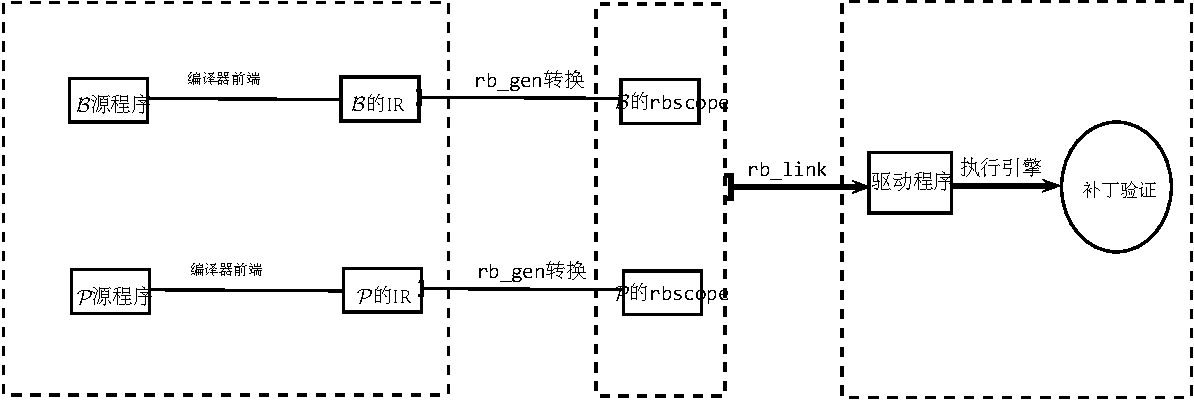
\includegraphics[width=.95\textwidth]{fig/workflow.pdf}\\
      {\scriptsize{\dryrun 的工作流}}
    \end{center}
  \end{figure}
\end{frame}

\begin{frame}
  \frametitle{\rbscope 的生成流程}
  \begin{columns}
    \column{.45\textwidth}
    \vspace{-30pt}
    \begin{figure}[t]
      \begin{center}
        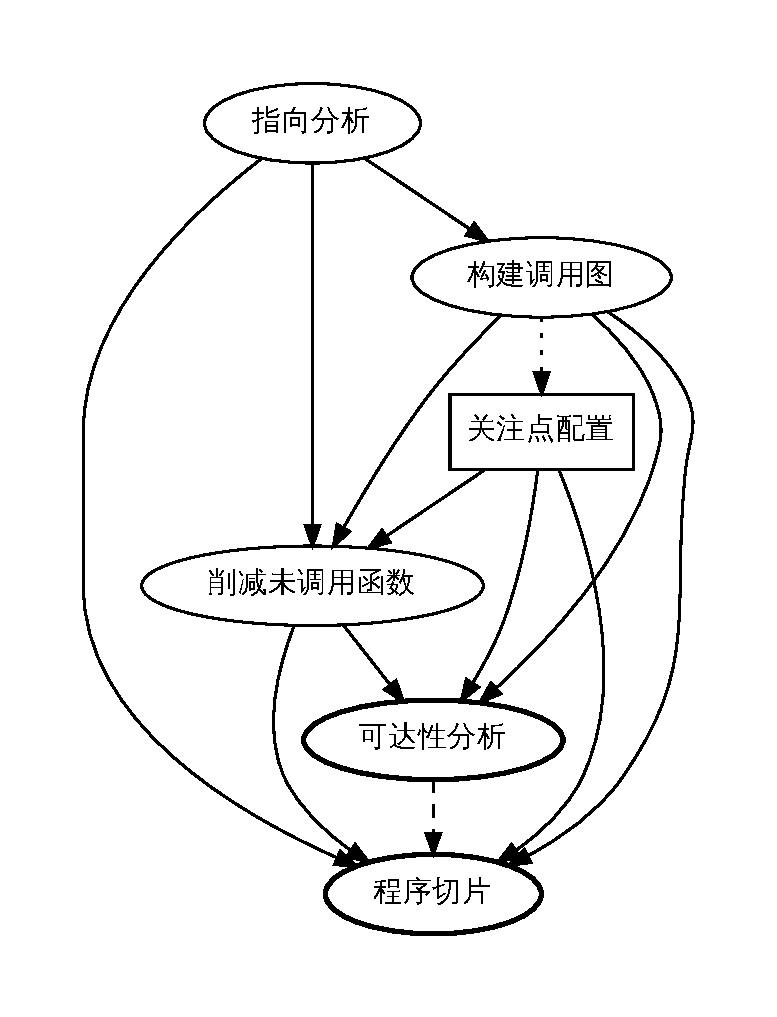
\includegraphics[height=.85\textheight]{fig/rb_gen.pdf}
      \end{center}
    \end{figure}
    \column{.45\textwidth}
    \pause
    \footnotesize{
      通过程序削减生成\rbscope 的过程需遵循下面的基本原则:
      \begin{itemize}
      \item[\ding{223}] 保留下的程序必须包含\structure{所有}可能执行的代码,即削减过程必须是保守的。
      \item[\ding{223}] 保留下的程序在添加了驱动程序之后必须是\structure{可执行}的。
      \item[\ding{223}] 出于选择性符号执行要求,削减程序过程应该尽可能\structure{精确}。
      \end{itemize}
    }
  \end{columns}
\end{frame}

% \label{sec:validate}
% \section{交叉验证}

\begin{frame}[containsverbatim]
  \frametitle{交叉验证的伪代码表示}
  \begin{columns}
    \column{.45\textwidth}
    \begin{lstlisting}[language={[ANSI]C}]
      int patch_error = 0, bug_error = 0;
      void cross_validate() {
        if (bug_error && patch_error)
        assert(0, "incomplete patch!");
        else if (bug_error && !patch_error)
        assert(0, "bug fixed!");
        else if (!bug_error && patch_error)
        assert(0, "regression patch!");
        else
        assert(0, "correct and no change!");
      }
      int main(void) {
        make_symbolic(symargs);
        buggyRB();
      }
    \end{lstlisting}

    \column{.45\textwidth}
    \begin{lstlisting}[language={[ANSI]C}]
      void patchedRB() {
        { // the rbscope of patched program
          ...
          patch_error = 1; // replace patch program assert
        }
        cross_Validate();
      }

      void buggyRB(void) {
        { // the rbscope of buggy program
          ...
          bug_error = 1; // replace bug program assert
          patchedRB();
        }
      }
    \end{lstlisting}

  \end{columns}
\end{frame}

\begin{frame}[<+-|alert@+>]
  \frametitle{\dryrun 的使用方法}
  \begin{itemize}
  \item[\ding{43}] 给定程序\prog ,通过提供的Emacs扩展将\prog\entry , \prog\bs , \prog\ps 信息写入配置文件config.json中。
  \item[\ding{43}] 将\prog 通过llvm-gcc(或clang)转换成LLVM的中间形式
  \item[\ding{43}] 装载LLVM的opt扩展rb\_gen,根据需要执行下面的转换
    \begin{enumerate}
    \item \textmd{rb-md} 将config.json中的信息以元数据形式写入LLVM的IR中
    \item \textmd{rb-uncall} 删除编译单元中未被调用函数
    \item \textmd{rb-reach} 分析对\prog\ps 和\prog\bs 的过程间可达性,并依此削减程序
    \item \textmd{rb-slice} 对得到的程序进行过程间切片
    \end{enumerate}
  \item[\ding{43}] 利用驱动程序合成工具\textmd{rb\_link},添加程序入口及符号执行语义,得到klee-input.bc
  \item[\ding{43}] 调用KLEE对klee-input.bc进行符号执行
  \end{itemize}
\end{frame}

\part{实验与评估}
\frame{\partpage}

\begin{frame}
  \frametitle{测试用例及\rbscope 生成}
  \begin{table}
    \centering
    \tiny
    \begin{tabular}{|c|c|c|c|c|c|c|c|}
      \hline
      编号 & 程序名 & \patch\ps & \patch\bs 行号 & 类型 & \patch\scope 大小(Kb) & $T_{rbc}$(ms)& \patch 大小(Kb) \\
      \hline
      01 & cut & 620 & 624 &  添加 &2.6 & 106 & 181\\ \hline
      02 & factor & 114 & 121 &  修改 & 2.2 & 62 & 139\\ \hline
      03 & join & 642 & 586 & 修改 & 1.8& 54& 168\\ \hline
      04 & mv & 461 & 465 &  修改 & 2.8 & 62 & 404 \\ \hline
      05 & od & 881 & 991 &  修改 & 2.0 & 60 & 193 \\ \hline
      06 & od & 1,290 & 1,389 &  修改 & 3.7 & 60 & 193\\ \hline
      07 & rm & 322 & 347 &  修改 & 1.8 & 71 & 257 \\ \hline
      08 & tail & 139 & 638 &  修改 & 2.7 & 89 & 210 \\ \hline
      09 & tr & 419 & 1,107 & 修改 & 2.1 & 56 & 187 \\ \hline
      10 & tr & 898 & 810 &  修改 & 8.9 & 55 & 187 \\ \hline
      11 & tr & 422 & 1,107 & 删除 & 2.2 & 54 & 187 \\ \hline
      12 & tsort & 140 & 170 &  修改 & 4.9 & 63 & 141 \\ \hline
    \end{tabular}
    \label{tab:cases}
  \end{table}
\end{frame}

\begin{frame}
  \frametitle{对补丁验证的可行性和高效性的评估}
  \vspace{-8pt}
  \begin{table}
    \centering
    \tiny
    \begin{tabular}{|p{0.80cm}|c|c|c|c|r|}
      \hline
      编号 & 版本 & 是否有效 & 验证时间(s)& 指令数(K) & 查询次数 \\
      \hline
      \multirow{2}{0.80cm}{01}
      & $rb\_scope$ &是 &  0.47  & 5.1 & 63  \\  \cline{2-6}
      & original &  否 & 超时 &   84,869.0 & 3,968  \\
      \hline
      \multirow{2}{0.80cm}{02}
      & $rb\_scope$ &否 & 0.49 & 6.2 & 120  \\  \cline{2-6}
      & original & 是 & 57.251 &  137.1 & 504  \\
      \hline
      \multirow{2}{0.80cm}{03}
      & $rb\_scope$ &否 & 1.09 & 9.8 & 69  \\  \cline{2-6}
      & original &  否 & 超时 &  1,433,000.1 & 4,319  \\
      \hline
      \multirow{2}{0.80cm}{04}
      & $rb\_scope$ &是 &  1046.17 & 1,027.4 & 4,121  \\  \cline{2-6}
      & original & 否 & x &  x & x  \\
      \hline
      \multirow{2}{0.80cm}{05}
      & $rb\_scope$ &是 &  26.80 & 6.7 & 338  \\  \cline{2-6}
      & original & 否 & 超时 &  363,301.0 & 1,983   \\
      \hline
      \multirow{2}{0.80cm}{06}
      & $rb\_scope$ &是 &  3.48 & 5.3 & 74  \\  \cline{2-6}
      & original & 否 &超时  & 276,434.2 & 7,0982  \\
      \hline
      \multirow{2}{0.80cm}{07}
      & $rb\_scope$ &是 &  1.02 & 5.5 & 77  \\  \cline{2-6}
      & original & 是 & 1.06 & 18.9   & 148  \\
      \hline
      \multirow{2}{0.80cm}{08}
      & $rb\_scope$ &是 &  1.80 & 5.2 & 60  \\  \cline{2-6}
      & original & 否 & 超时 &  2,422,569.1 & 270  \\
      \hline
      \multirow{2}{0.80cm}{09}
      & $rb\_scope$ &是 &  3.41 & 18.5 & 79  \\  \cline{2-6}
      & original & 否 & 超时 &  245.7 & 775  \\
      \hline
      \multirow{2}{0.80cm}{10}
      & $rb\_scope$ &是 &  2.64 ms & 6.1 & 13  \\  \cline{2-6}
      & original & 是 & 672.69  &  1,299.6 & 3,021  \\
      \hline
      \multirow{2}{0.80cm}{11}
      & $rb\_scope$ &是 &  20.13 & 2.3 & 838  \\  \cline{2-6}
      & original & 否 & 超时  &  4,521.9 & 8,432  \\
      \hline
      \multirow{2}{0.80cm}{12}
      & $rb\_scope$ &是 &  3.02 & 5.5 & 88  \\  \cline{2-6}
      & original & 否 & 超时 &  4,651.3 & 4,648  \\
      \hline
    \end{tabular}
    \label{tab:eval1}
  \end{table}
\end{frame}

\begin{frame}
  \frametitle{对回归错误和错误肯定的评估}
  \begin{table}
    \centering
    \tiny
    \begin{tabular}{|l|c|c|c|r|}
      \hline
      编号 & \footnotesize{Regression} & $T_{cv}$(s) & \footnotesize{FP} &$T_{fp}$(s) \\
      \hline
      01 & 是 & 1.08 & 否 & 0.79 \\ \hline
      02 & - & 超时 & - &超时\\ \hline
      03 & 是 & 1.09 & 否 &5.64\\ \hline
      04 & - & 超时 & - &超时\\ \hline
      05 & - & 超时 & - &超时\\ \hline
      06 & 是 & 114.54 & 否 & 540.84\\ \hline
      07 & 否 & 9.17 & 是 & 2.09\\ \hline
      08 & 否 & 7.26 & 否 & 8.50\\ \hline
      09 & 是 & 2.01 & 否 & 8.03\\ \hline
      10 & - & 超时 & - &超时\\ \hline
      11 & 是 & 2.11 & 否 & 93.40\\ \hline
      12 & 是 & 3.02 & 否 & 7.94\\ \hline
    \end{tabular}
    \label{tab:eval2}
  \end{table}
\end{frame}

\part{总结与展望}
\label{part:summary}
\frame{\partpage}

\begin{frame}
  \frametitle{总结}
  本文在开源编译器框架LLVM、符号执行引擎KLEE及STP约束求解器的基础上实现了反映上述想法的工具原型\dryrun 。从GNU Coreutils程序集合选取了数十个补丁程序对它进行评估,\dryrun 成功地找出了所有不正确补丁; 同时,和KLEE对完整的程序执行相比,检测程序中的错误的性能大大提高, 速度上最高有1000倍的提升。这样的结果说明通过剔除不相关代码而有选择地进行符号执行的思路是可行的。
\end{frame}

\begin{frame}
  \frametitle{缺陷与不足}
\end{frame}

\begin{frame}
  \frametitle{未来的改进}
  \begin{itemize}
  \item[\ding{47}] 结合LLVM提供的编译优化,优化Andersen指向分析算法的实现
  \item[\ding{47}] 在程序依赖图上采用更精确的过程间切片
  \item[\ding{47}] 通过静态分析的方法得到程序执行到\rbscope 时的最弱前置条件给出符号变量的上下界
  \item[\ding{47}] 不直接削减程序本身而采用添加注解(annotation)的方式标记程序中的\rbscope ,并以此修改KLEE执行方式
  \item[\ding{47}] 使用\textbf{$S^2E$}等扩展性更好的符号执行框架
  \end{itemize}
\end{frame}

% \appendix
% \newcount\opaqueness
% \begin{frame}
%   \begin{centering}
%     \Huge\color{green!60!black} 谢谢各位老师!\par
%   \end{centering}
% \end{frame}

\end{document}